\chapter{Indexers and Well Configuration}
\index{Indexers}\index{Data ingest}
The two core components of a Gravwell deployment are the Indexer and
Webserver. If either of those components are not properly configured,
Gravwell will not function. The indexer is the most important
component, as it is responsible for actually storing, maintaining, and
querying data. ~In this section we will examine the role of a Gravwell
indexer and how to appropriately configure and debug it.

Gravwell follows the principle of least privilege: the shell and Debian
installers will create an unprivileged user and group named
\code{gravwell}. Gravwell files and resources are stored in
\code{/opt/gravwell} which is owned by the \code{gravwell} user. Most
components have no special permissions and cannot affect sensitive
system files. The exceptions are the webserver, simple relay ingester,
file follower ingester, and PCAP ingester. The webserver and simple relay ingesters are given the
\code{CAP\_NET\_BIND\_SERVICE}\footnote{http://man7.org/linux/man-pages/man7/capabilities.7.html} capability which allows them to bind to low ports; this is so we can serve web pages
on ports 80 and 443 and listen for syslog packets on ports 514 and 601. The file follower ingester has a default systemd
unit file which starts the process under the user \code{gravwell} and group
\code{adm},which allows it to access typical file based system logs in
\code{/var/log}. The PCAP ingester is given the
\code{CAP\_NET\_RAW} capability so that it can bind to raw
sockets\footnote{https://en.wikipedia.org/wiki/Network\_socket\#Raw\_socket}. The
special groups or capabilities can be removed, but the webserver will
not be able to bind to low ports and the file follower ingester may not
be able to read system logs.


\section{Indexer Configuration}
\index{gravwell.conf@\code{gravwell.conf}}
Gravwell always ships with a functional gravwell.conf that provides a
basic deployment right out of the box. However, with very large or very
complex deployments, tuning the configuration can yield much better
performance and stability. Both indexers and webservers can share the
same configuration file, which is located at
\code{/opt/gravwell/etc/gravwell.conf} by default. The configuration file
that is shipped in a typical Gravwell installer is very minimal and
represents a basic configuration. The shell installer and Debian
package both contain logic to inject randomly generated tokens into each
required authentication parameter. The published Docker image on Docker
Hub\footnote{https://hub.docker.com/} contains
environment variables preconfigured to set the authentication tokens.\index{Docker}
The preconfigured environment variables for the Docker deployment are
not unique and not secure. If you plan to use Gravwell in Docker, you
must override these configuration values using either Docker secrets or
custom values.

\subsection{Hands-on Lab: Misconfigured Indexer}
\label{sec:MisconfiguredIndexer}

For this hands on lab we will be deploying a slightly misconfigured
Gravwell instance. We will examine error logs to identify the
misconfiguration and correct it. To get started, let's cd to the
working directory in our training folder named \code{Indexers/Lab-MisconfiguredIndexer}:

\code{cd \textasciitilde{}/gravwell\_training/Indexers/Lab-MisconfiguredIndexer}

Next, follow the steps to get your misconfigured Gravwell instance up
and running:

\begin{enumerate}

\item Create a gravwell container using the \code{gravwell:base} image
\begin{Verbatim}[breaklines=true]
docker create --name test --net gravnet gravwell:base
\end{Verbatim}

\item Copy the \code{gravwell.conf} file into the container
\begin{Verbatim}[breaklines=true]
docker cp config/gravwell.conf test:/opt/gravwell/etc/
\end{Verbatim}

\item Start the container

\begin{Verbatim}[breaklines=true]
docker start test
\end{Verbatim}

\item Get the container IP address
	\begin{Verbatim}[breaklines=true]
docker inspect --format \
'{{.NetworkSettings.Networks.gravnet.IPAddress}}' test
	\end{Verbatim}

\item Obtain a shell within the container
\begin{Verbatim}[breaklines=true]
docker exec -it test /bin/sh
\end{Verbatim}

\end{enumerate}

\subsubsection{Lab Questions}

\begin{enumerate}
\item
  {Are you able to view the Gravwell web portal?}

\item
  {Is the indexer process running?}

\item
  {What log files are available to identify the problem?}

\item
  {Why couldn't the indexer start?}

\item
  {What parameter in the gravwell.conf caused the failure?}

\item
  {What is the default value for the parameter and how would you change
  it?}
\end{enumerate}

\subsubsection{Hands-on Lab Tips and Solutions}

If a Gravwell instance is failing to respond, the first item of
business is to identify whether or not the Gravwell processes are
running. All Gravwell processes are prefixed with \code{gravwell\_} so we
can issue a \code{ps \textbar{} grep gravwell} to get a list of running
gravwell processes. In your container you should see the
\code{gravwell\_webserver} and \code{gravwell\_searchagent} process, but \emph{not}
\code{gravwell\_indexer}.

\begin{Verbatim}[breaklines=true]
/ # ps | grep gravwell_
11 root    0:00 /opt/gravwell/bin/gravwell_webserver -stderr webserver
13 root    0:00 /opt/gravwell/bin/gravwell_searchagent -stderr searchagent
45 root    0:00 grep gravwell_
\end{Verbatim}

The indexer logs status information to a standard set of logs in
\code{/opt/gravwell/log}, but if the process encounters a critical failure
that prevents it from writing to the standard log files, it will write
to a file in \code{/dev/shm/}. When a gravwell process fails and exits it
will attempt to write the reason in \code{/opt/gravwell/log/error.log}, so
check the error log to see if there is a message indicating the problem.
Run \code{tail /opt/gravwell/log/error.log} and you should see something
like:

\code{03-14-2019 22:35:27.185 {[}8000020b{]} backend/main.go:561 Failed to
create the search server: listen tcp :4023: bind: address already in
use}

This message indicates that the Gravwell indexer process could not bind
to port 4023 because something else was already bound to that port. The
search server is the component within the Gravwell indexer that responds
to commands from the webserver. The configuration parameter that
controls which port it binds to is \code{Control-Port}. Open the
gravwell.conf file you retrieved from the training server and examine
its contents.

Let's change the \code{Control-Port} value to its default of 9404, copy
the configuration file back into the container and restart it:


\begin{Verbatim}[breaklines=true]
docker cp gravwell.conf test:/opt/gravwell/etc/
docker restart test
\end{Verbatim}

You should now be able to log into the gravwell web portal using the IP
address discovered earlier. Do not \code{rm} the test container, as we are
going to use it again for the next lab.

\section{Well Configuration}
\index{Wells}
Properly configuring a well can yield significant performance gains
when querying data. Isolating data into different wells means that when
you issue a query on a tag, the indexer can look at storage that is only
associated with that tag. This allows for highly tuned configurations
and storage arrangements. For example, let's assume that your Gravwell
instance is consuming firewall logs, syslog, Netflow v5, and packet
capture. The logs and Netflow may represent a few gigabytes of data per
day and may have retention requirements, where the packet capture might
produce hundreds or thousands of gigabytes per day and have no retention
requirements. So while it might be very useful to consume packet data
and hold it for a short time, it is not subject to the same rules or
priority as the logs. Isolating it into its own well means that the
high volume of packet data will have minimal impact on the logs and
Netflow, and can be managed very differently.

To add a new well for an indexer we will need to add the well
definition and associate the tag with it. Let's look at a well
definition named ``raw'' that stores data in
\code{/opt/gravwell/storage/raw} and is responsible for all entries with
the tag \code{pcap} and \code{binary}: 

\begin{Verbatim}[breaklines=true]
[Storage-Well "raw"]
    Location=/opt/gravwell/storage/raw
    Tags=pcap
    Tags=binary
\end{Verbatim}

We can define as many wells as you would like; the only requirement is
that every well must have its own storage location and none of the
assigned tags may overlap. For example, the tag \code{pcap} cannot be
assigned to multiple wells, and two different wells cannot use the same
storage directory. If a well specifies a storage location that does not
exist, it will attempt to create it. However, because the indexer is
typically running as a restricted user it may not be able to. If you
are specifying well storage locations outside of
\code{/opt/gravwell/}, ensure that the location already exists and has the
appropriate permissions. It should be owned by the user/group
\code{gravwell/gravwell} and have RWX permissions enabled for the owner.

\subsection{Hands-on Lab: Well Definitions}

{For this lab we are going to modify the }{gravwell.conf}{~file to
include a new well definition. ~We will use the existing container from
the previous lab ("Misconfigured Indexer", \ref{sec:MisconfiguredIndexer})

Open the gravwell.conf file you fixed in the previous lab and append the
following well definition:

\begin{Verbatim}[breaklines=true]
[Storage-Well "syslog"]
    Location=/opt/gravwell/storage/syslog
    Tags=syslog
\end{Verbatim}


{The entire gravwell.conf file should be:

\begin{Verbatim}[breaklines=true]
[global]
### Web server HTTP/HTTPS settings
Web-Port=80
Insecure-Disable-HTTPS=true

### Other web server settings
Remote-Indexers=net:127.0.0.1:9404

### Ingester settings
Ingest-Port=4023
Control-Port=9404

### Other settings
Log-Level=INFO
Pipe-Ingest-Path=/opt/gravwell/comms/pipe

### Paths

[Default-Well]
        Location=/opt/gravwell/storage/default/

[Storage-Well "syslog"]
        Location=/opt/gravwell/storage/syslog
        Tags=syslog
\end{Verbatim}

Now copy it into the test container and restart the container:

\begin{Verbatim}[breaklines=true]
docker cp gravwell.conf test:/opt/gravwell/etc
docker restart test
\end{Verbatim}

Obtain a shell within the docker container (\code{docker exec -it test
/bin/sh}) and check that the indexer process started, and that the well
storage location was created. You should see some shards already in the
storage folder.

\begin{Verbatim}[breaklines=true]
user@training:~/gravwell_training$ docker exec -it test /bin/sh
/ # ps -o pid,comm
PID   COMMAND
    1 manager
   11 gravwell_webser
   13 gravwell_search
   18 gravwell_indexe
   55 sh
   60 ps
/ # ls -al /opt/gravwell/storage/default/
total 8
drwxr-x---    2 root     root          4096 Mar 24 20:17 .
drwxr-x---    8 gravwell gravwell      4096 Mar 24 20:17 ..
/ #
\end{Verbatim}

We can also validate that the new well was created within the GUI,
expand the left sidebar navigation menu and click ``Wells \& Indexers''.
You should see two wells, default and syslog, as shown in Figure \ref{fig:wells}

\begin{figure}
	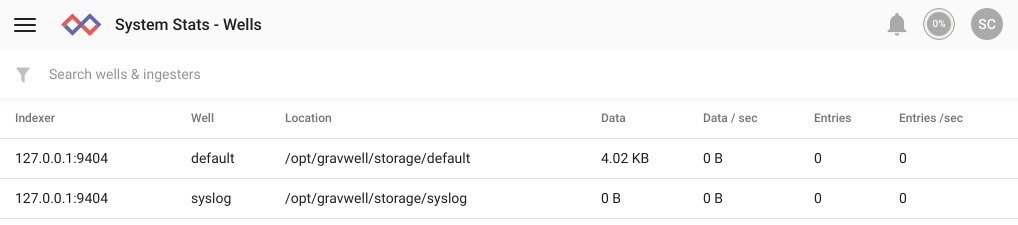
\includegraphics{images/wells.png}
	\caption{Wells and Indexers}
	\label{fig:wells}
\end{figure}

{The indexer also automatically created the syslog tag when it found the
new well configuration. You can click the tags menu item and see that
Gravwell now knows about the }{syslog}{~tag, enabling you to search with
it. ~There are no entries yet, as we haven't ingested anything, but the
tag is there.}

\begin{figure}
	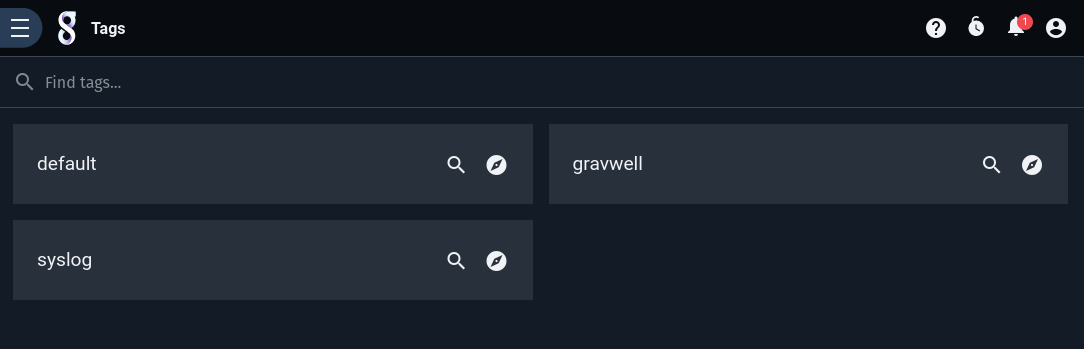
\includegraphics{images/tags.png}
	\caption{Tags}
\end{figure}

Do not \code{rm} the test container, as we are
going to use it again for the next lab.

\section{Well Ageout}
\index{Ageout}\index{Wells!ageout}
Gravwell is designed to manage data sets with minimal user interaction;
once a system is appropriately configured it will manage data sets and
storage arrays on its own. Data ageout is one of the most critical
configurations. Properly configured well ageouts prevent disk
exhaustion, enable high speed working datasets, and allow for regulatory
or retention compliance. This section will examine the available
rulesets which control how Gravwell indexers manage stored data and how
we can use multi-tiered storage to adhere to compliance requirements
while still utilizing a smaller pool of high speed storage for
day-to-day operations.

Data ageout can be controlled using three different constraints: time,
total storage, and storage availability. Ageout is also configured on a
per well basis, so each well can have entirely different ageout rules.
The per well ageout rules enable Gravwell administrators to prioritize
data and adhere to corporate or regulatory requirements without lumping
every data source into the same rule set or priority. Data that must be
captured but may not be useful in day to day operation can be stored
directly on low-cost storage devices for long term storage. Data that
may not have legal or corporate retention requirements but plays a
central role in network management or security operations can use high
speed storage and ageout to low-cost storage as needed. Gravwell ageout
rules provide a tremendous amount of flexibility in managing how data is
stored.

Gravwell indexers are very sensitive to data deletion. You
\emph{must} explicitly enable data deletion via the ageout controls using
the \code{Delete-Cold-Data} and \code{Delete-Frozen-Data} parameters. If the
respective parameters are not set to ``true'', an indexer will not
delete data, even if the other configuration parameters indicate that it
should. This additional configuration parameter is somewhat like a
secondary sanity check, forcing you to fully acknowledge that Gravwell
is allowed to delete data.

\textbf{WARNING}: Data ageout operates on entire shards and ageout constraints
must be satisfied by an entire shard before an ageout executes. A
typical shard size is 1.55 days, so if you set a time based ageout of 1
day, Gravwell won't perform an ageout until \emph{all} data in a shard is
more than 1 day old. This means that even though you specified an
ageout duration of 1 day, the storage tier will hold up to 1.55 days.
When an ageout occurs, the entire shard is aged out at once.

\subsection{Time-based Ageout}

Time-based ageout uses entry timestamps to determine their life cycle.
Ageout is specified using time spans that define retention durations.
Each storage tier can maintain an independent duration configuration.
For example, we can define that entries are held in the hot storage
pool until they are greater than 30 days old, at which point they are
deleted or moved to a cold storage tier. Cold storage can then specify
that data be held for 120 days before it is deleted or archived.
Time-based retention is controlled by the \code{Hot-Duration} and
\code{Cold-Duration} well parameters. Durations can be specified in days
(d) or weeks (w). Because aging out data incurs some computation and
storage costs, it may be beneficial to schedule the ageout for a time of
day when users are not interacting with Gravwell, or when log data
volumes are lower. The \code{Ageout-Time-Override} parameter allows you to
set the time of day that the time-based ageouts occur--note that
this time is specified in UTC!

Below is an example well configuration that stores data in the hot tier
for seven days, then moves it to the cold tier where it is held for 16
weeks and then deleted. Ageout occurs at 1AM UTC.

\begin{Verbatim}[breaklines=true]
[Default-Well]
        Location=/mnt/ssd/gravwell/default/
        Cold-Location=/mnt/hdd/gravwell/default
        Hot-Duration=7d
        Cold-Duration=16w
        Delete-Frozen-Data=true
        Ageout-Time-Override="1:00"
\end{Verbatim}

This is a well that does not maintain a cold storage tier; instead it simply
deletes data once it is 90 days old:

\begin{Verbatim}[breaklines=true]
[Default-Well]
        Location=/opt/gravwell/storage/default/
        Hot-Duration=90d
        Delete-Cold-Data=true
\end{Verbatim}

\textbf{WARNING}: The indexer host clock is critically important for accurate
ageout controls.~The timestamps on entries are entirely decoupled from
the time on the host indexer. If you misconfigure the host clock on an
indexer, ageout may execute prematurely, or not at all.

\subsection{Storage-based Ageout}

Storage-based ageout uses the total physical storage consumed to
determine data lifecycles. Using storage-based ageout is convenient
when managing smaller high-speed storage pools, managing specific
storage usage, or when there are no retention requirements. Wells
configure their storage-based ageouts using the
\code{Max-Hot-Storage-GB} and \code{Max-Cold-Storage-GB} well parameters.
Setting a storage constraint tells Gravwell that if a well storage tier
goes over the specified storage limit, it should attempt an ageout
immediately. Storage-based ageout rules operate entirely independently
of time-based rules. If both time- and storage-based ageouts are
configured and the storage tier exceeds the configured storage limit,
the indexer will attempt an ageout regardless of what the time-based
controls say.

This is a well configured with two storage tiers. The hot tier is
configured to hold 10GB and the cold tier is configured to hold 100GB,
so the entire well will hold 110GB of searchable data:

\begin{Verbatim}[breaklines=true]
[Default-Well]
        Location=/mnt/ssd/gravwell/default/
        Cold-Location=/mnt/hdd/gravwell/default
        Max-Hot-Storage-GB=10
        Max-Cold-Storage-GB=100
        Delete-Frozen-Data=true
\end{Verbatim}

This is a well configured to use a storage constraint on the hot tier
and a time constraint on the cold tier. This means it will keep 10GB in
the hot storage device, but ensure that data is held for at least 90
days using the cold storage device:

\begin{Verbatim}[breaklines=true]
[Default-Well]
        Location=/mnt/ssd/gravwell/default/
        Cold-Location=/mnt/hdd/gravwell/default
        Max-Hot-Storage-GB=10
        Cold-Duration=90d
        Delete-Frozen-Data=true
\end{Verbatim}

\textbf{WARNING}: Data ageout can take non-zero time. Ensure that you have
ample storage space to continue ingesting new data while old data is
moved between storage tiers. For example, if your hot storage tier has
128GB of available storage it is wise to configure the storage limit to
120GB so that you have 8GB of slack available while the ageout is in
progress.

\subsection{Storage Availability Ageout}

Storage availability-based ageout a highly flexible system which
enables indexers to use storage without hard constraints on time or
stored data. The availability constraints are used to define a specific
percentage of storage that the indexer \emph{cannot} use, a sort of reserve
space. The constraints are controlled by the
\code{Hot-Storage-Reserve} and \code{Cold-Storage-Reserve} parameters.
Storage reserves are calculated by each well and storage tier
independently. This means that wells do not coordinate with each other
and they do not treat disk usage by outside applications any differently
than storage used by Gravwell.

This is a well definition which maintains a 10\% reserve on the hot
storage tier:

\begin{Verbatim}[breaklines=true]
[Default-Well]
        Location=/opt/gravwell/storage/default/
        Hot-Storage-Reserve=10
        Delete-Cold-Data=true
\end{Verbatim}

This is a configuration with two wells, both using storage
reserve-based constraints. Notice that both wells are based in
\code{/opt/gravwell/storage/}; if we assume that storage locations are on
the same storage device the ageout behavior may be unexpected. For
example, if the storage device has 128GB of available storage, and the
default well has shards that are 100GB in size while the syslog well has
shards that are 1GB in size it will be extremely difficult to predict
which well will actually delete its data. If the default well
triggers first, the syslog well may be able to maintain months worth
of data. If the syslog well triggers first it may delete all of its
shards trying to hit the storage reserve.

\begin{Verbatim}[breaklines=true]
[Default-Well]
        Location=/mnt/ssd/gravwell/default/
        Hot-Storage-Reserve=10
        Delete-Cold-Data=true

[Storage-Well "syslog"]
        Location=/opt/gravwell/storage/syslog
        Tags=syslog
        Hot-Storage-Reserve=20
        Delete-Cold-Data=true
\end{Verbatim}

\textbf{WARNING}: Using the availability constraints when a Gravwell indexer
does not have exclusive control over an entire storage device can yield
unexpected ageout behavior.

\subsection{Hands-on Lab: Ageout}

This hands-on lab will continue to use the Gravwell docker instance
that we used in the previous labs. We are going to apply ageout
constraints to the \code{default} and \code{syslog} wells and watch data move
from the hot tier to the cold tier. First, let's make sure our previous
container is running, then change to the \code{Lab-Ageout} directory in
our training folder:

\begin{Verbatim}[breaklines=true]
docker start test
cd ~/gravwell_training/Indexers/Lab-Ageout
\end{Verbatim}

Then we'll use the ingesters container (make sure you've loaded the ingesters container image as described in Section \ref{sec:load-lab-images}) to import the syslog data:
\begin{samepage}
\begin{Verbatim}[breaklines=true]
docker run -v $PWD/data:/tmp/data --rm -i --net gravnet \
gravwell:ingesters /opt/gravwell/bin/reimport -rebase-timestamp \
-clear-conns test:4023 -i /tmp/data/syslogdata -import-format json
\end{Verbatim}
\end{samepage}

In the command above, we spin up a new container and run the \code{reimport} ingester, telling it to read json-formatted entries from standard input.

Next, let's apply some ageout constraints to the two wells. We have provided a copy of the
base gravwell.conf in the config/ subdirectory, so modify it and add the following constraints:

\begin{enumerate}
	\item \code{Default well}
	\begin{enumerate}
		\item{One storage tier}
		\begin{enumerate}
			\item Hot is at /opt/gravwell/storage/default
		\end{enumerate}
		\item Hot tier holds 14 days of data
		\begin{enumerate}
			\item Data is deleted after
		\end{enumerate}
	\end{enumerate}
	\item Syslog well
	\begin{enumerate}
		\item Two storage tiers
		\begin{enumerate}
			\item Hot location is /opt/gravwell/storage/syslog
			\item Cold is at /opt/gravwell/cold\_storage/syslog
		\end{enumerate}
		\item Hot tier holds 7 days of data
		\item Cold tier holds 1GB
		\begin{enumerate}
			\item Data is deleted after
		\end{enumerate}
	\end{enumerate}
\end{enumerate}

Once you have made your docker configuration changes copy the
configuration file into the test container and start it.

\begin{Verbatim}[breaklines=true]
docker cp config/gravwell.conf test:/opt/gravwell/etc/
docker restart test
\end{Verbatim}

Check the ``Wells \& Indexers'' page on the GUI to verify that your
indexer is properly configured. You should see about 20k entries in the
\code{syslog} well in hot storage.

\begin{figure}
	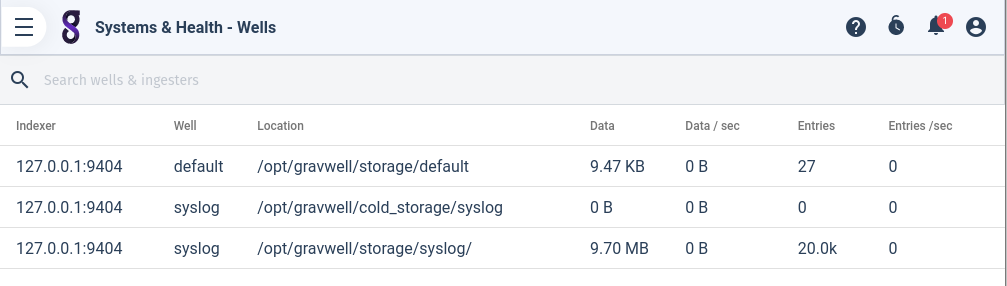
\includegraphics{images/hotstore.png}
	\caption{Data in Hot Store}
\end{figure}

In a few minutes, the indexer will age the hot data into the cold
well.

\begin{figure}
	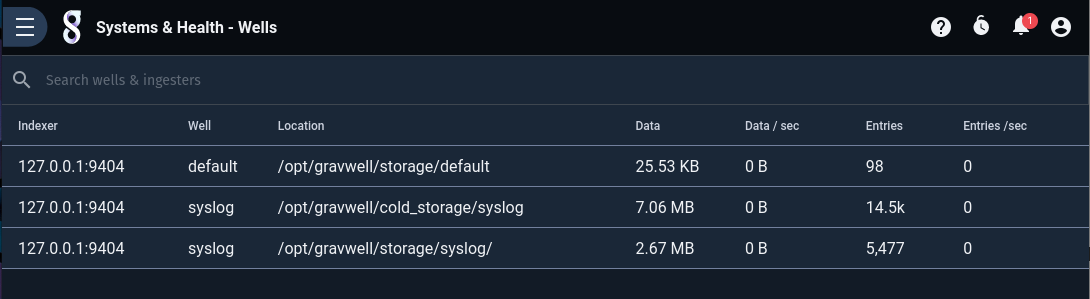
\includegraphics{images/coldstore.png}
	\caption{Data in Hot and Cold Stores}
\end{figure}

Your modified \code{gravwell.conf} well definitions should look something
like this:

\begin{Verbatim}[breaklines=true]
[Default-Well]
    Location=/opt/gravwell/storage/default/
    Hot-Duration=14d
    Delete-Cold-Data=true

[Storage-Well "syslog"]
    Location=/opt/gravwell/storage/syslog/
    Cold-Location=/opt/gravwell/cold_storage/syslog
    Tags=syslog
    Hot-Duration=7d
    Max-Cold-Storage-GB=1
    Delete-Frozen-Data=true
\end{Verbatim}

To clean up after the experiment, simply run:

\begin{Verbatim}[breaklines=true]
docker kill $(docker ps -a -q)
\end{Verbatim}

\section{Replication}
\index{Replication}
Hardware failures happen, drives crash, and humans mis-type commands;
only a robust data backup solution can prevent catastrophic data loss.
Gravwell implements a data replication system which enables transparent
data backup. As data is ingested, Gravwell will automatically assign
the data stream to a remote peer and copy the data shards to it. The
replication system is extremely flexible, enabling tolerance to node,
rack, and even data center failures. Indexers replicate data shards and
tag mappings, which is sufficient to completely rebuild a node in case
of total storage failure. Indexer configurations are not replicated, so
maintaining an up-to-date \code{gravwell.conf} file is important.}

This section will explore the two data replication mechanisms supported
by Gravwell and examine the pros and cons of each. We will describe how
to enable replication, pick peers, and recover from failures.
Replication is enabled for every paid Gravwell license, but Community
Edition licenses cannot enable replication.

\textbf{WARNING}: The \code{Indexer-UUID} variable in the gravwell.conf file is
used as the indexer identity in the replication group. When restoring
an indexer, it is critically important that you restore the correct UUID
prior to starting the indexer.

\subsection{Offline Replication Configuration}

Replication is entirely controlled by indexers. While webservers are
aware of indexer configurations and can request hot failover during
search, they do not have control over or insight into replication state
or peer selection. To enable replication, we add a replication
configuration block to the indexer's \code{gravwell.conf} file. Below is
an example replication configuration with a single offline replication
peer:

\begin{Verbatim}[breaklines=true]
[Replication]
    Peer=172.17.0.3
    Storage-Location=/opt/gravwell/replication_storage
    Disable-TLS=true
    Connect-Wait-Timeout=60
    Disable-Server=true
\end{Verbatim}

Notice that we disabled the server, but still specified a
Storage-Location; replication needs to store the state of replicated
data. While our server may not be replicating data from other nodes, it
still needs to track how much of its own data has been replicated.

There are a few important security considerations associated with the
above config:

\begin{enumerate}
	\item \code{Replication-Secret-Override}is not specified.
	\begin{enumerate}
		\item The indexer will use the \code{Control-Secret} for authentication.
	\end{enumerate}
	\item TLS is disabled, which means that indexer is using a cleartext connection.
	\begin{enumerate}
		\item Data is replicated in the clear and restored in the clear
	\end{enumerate}
	\item \code{Connect-Wait-Timeout=60} means Indexers will wait up to 60 seconds for a replication peer.
	\begin{enumerate}
		\item If an indexer cannot connect to a replication peer in that time, it will start.
		\item This is important when recovering from a failure.
		\item When restoring a failed node, it is recommended that this setting be 0, meaning the indexer will wait for a replication peer indefinitely before starting.
	\end{enumerate}
\end{enumerate}

\subsection{Hands-on Lab: Replication}

We will be instantiating an offline replication server and configuring
our test container to replicate data to it. The offline replication
server acts as a remote data store of replicated data and will allow our
indexer to recover from failure and re-import its data. After
replicating the data from our test instance we will destroy it and start
over. When the indexer comes back online, it will identify the failure
and restore its data and tag set from the replication server.

\subsubsection{Starting the Offline Replication Server}

Change your current working directory to \code{gravwell\_training/Indexers/Lab-Replication} and
check its contents. You should see a gravwell.conf file in the \code{config/} subdirectory. Make sure you've got the \code{offlinereplication} image loaded as described in Section \ref{sec:load-lab-images}, then start it with a name and hostname of
\code{offlineserver}:

\begin{Verbatim}[breaklines=true]
docker run -d --net gravnet --name offlineserver \
-h offlineserver gravwell:offlinereplication
docker ps
\end{Verbatim}

Next, stop your test container and edit the gravwell.conf to include a
replication configuration block so that it can replicate its data to the
offline replication server. We can use the hostname
\code{offlineserver} for the replication peer and leave the authentication
secrets blank for reasons that will be covered in section \ref{sec:docker-config}. Once you
are happy with your replication configuration block, copy it into the
test container and restart it. Then use ping and netstat to verify that the indexer has connected to the offline replication server:

\begin{Verbatim}[breaklines=true]
docker cp config/gravwell.conf test:/opt/gravwell/etc/
docker restart test
docker exec -it test ping -c 1 offlineserver
docker exec -it test netstat -pa | grep ESTABLISHED
\end{Verbatim}

We should see an established connection to the host
\code{offlineserver} on port 9406 (the replication port). Get a shell
on the offline replication server using \code{docker exec -it offlineserver
/bin/sh}. Print the replication configuration file to find the
replication storage directory, then navigate to that directory. We
should see a \code{replication.db} file and a directory with the same name
as our indexer's UUID. This means the indexer has connected and is
pushing shards to the offline replication server. Wait a few minutes
and watch as the indexer pushes each successive data shard to the
replication server.

Once the indexer has pushed all its shards (you should see about 20),
exit the offline replication server shell with the \code{exit} command.

Next, let's simulate a disk failure by destroying all the shards in our
indexer and restarting it. Let's start smashing some storage locations
within our indexer, then restart it:

\begin{Verbatim}[breaklines=true]
docker exec test rm -rf /opt/gravwell/storage/
docker exec test rm -rf /opt/gravwell/cold_storage/
docker restart test
\end{Verbatim}

These docker commands basically reached in and annihilated all the data
in our indexer and then restarted the entire container. If not for the
replication system we would have lost everything. However with
replication, if we wait just a moment we can see the indexer repopulate
its shards, ready for searching. You may have noticed that the
replication system restored the shards to the cold pool. The
replication system will typically target cold pool for restoration, only
pushing current hot shards to the hot pool.

\begin{figure}
	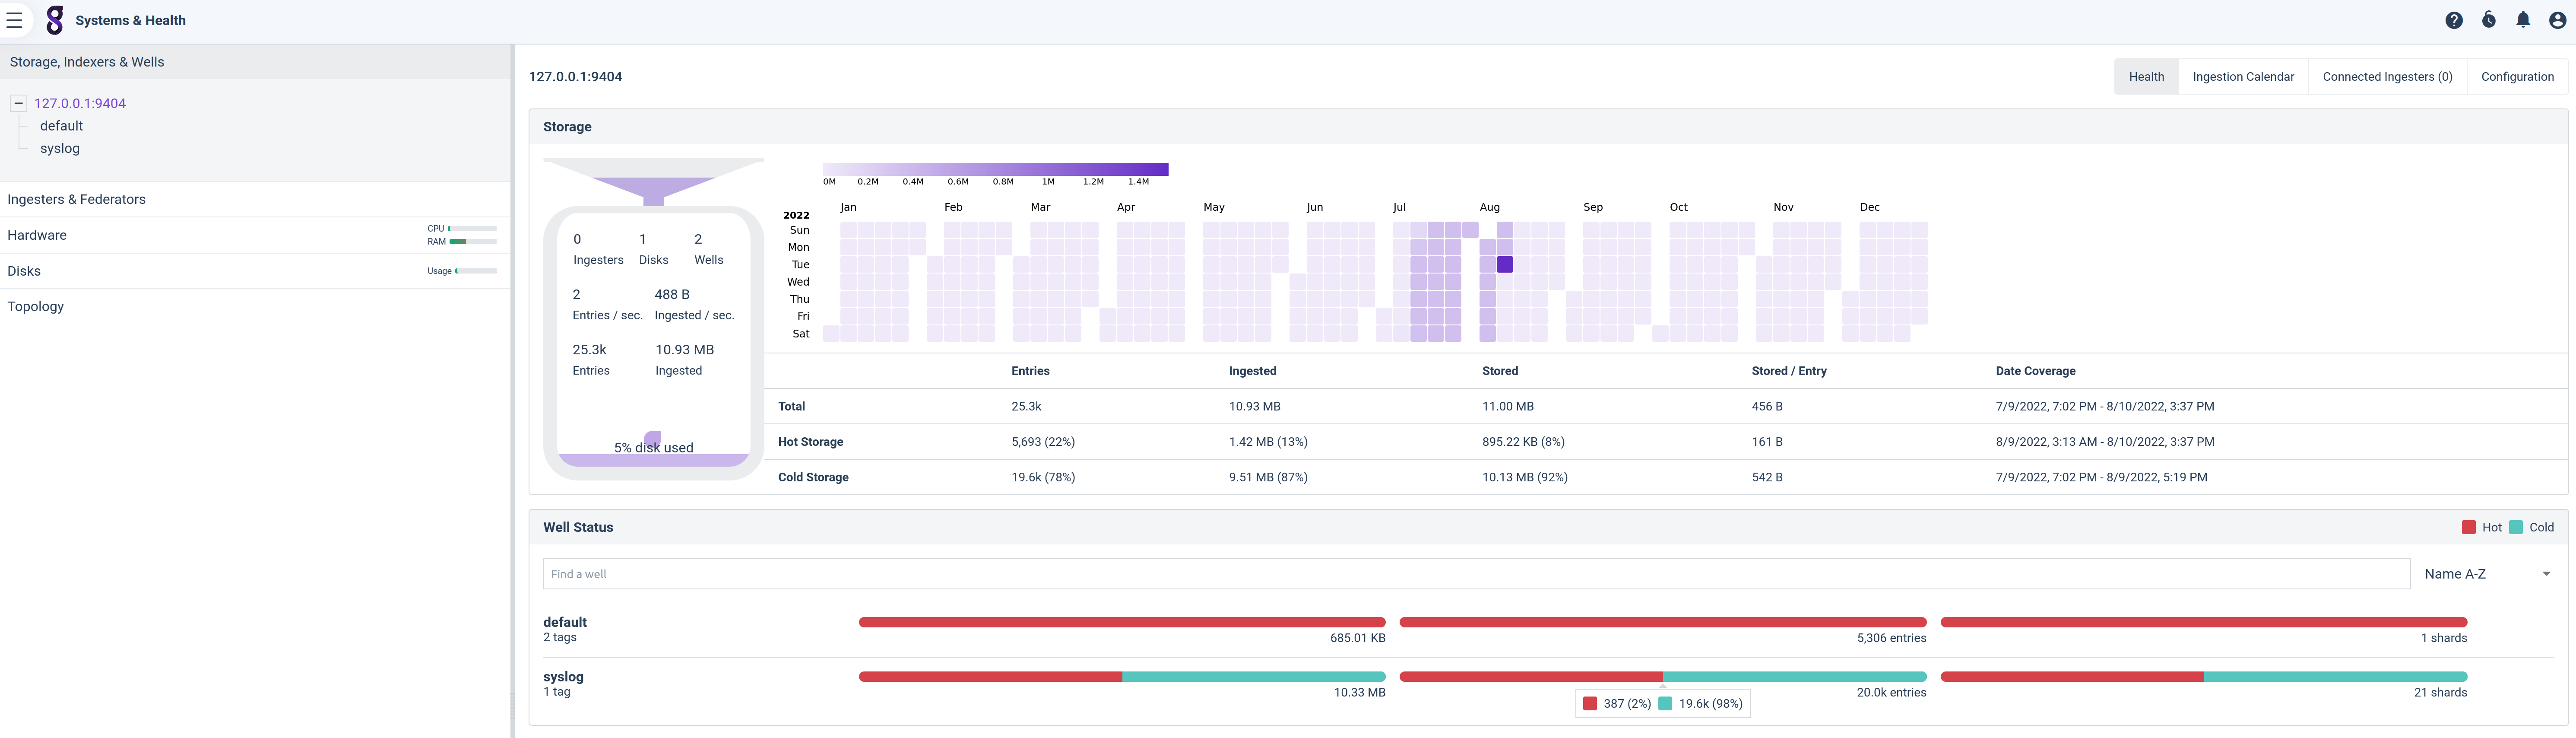
\includegraphics{images/replication-restore.png}
	\caption{Post-restoration Well Stats}
\end{figure}

\subsubsection{Lab Questions}

\begin{enumerate}
	\item Did the shard size change on the indexer after it was restored?
	\begin{enumerate}
		\item Why?
	\end{enumerate}
	\item Why would we want to restore shards to the cold well on replication recovery?
\end{enumerate}

To clean up after the experiment, simply run:

\begin{Verbatim}[breaklines=true]
docker kill $(docker ps -a -q)
\end{Verbatim}

\section{Query Acceleration and Indexing}
\label{sec:acceleration}
\index{Acceleration}\index{Indexing|see {Acceleration}}
Gravwell indexers provide a couple different data management
methodologies, ranging from raw storage with only temporal indexing to
full feature extraction with direct data indexing. This section
will explore indexer acceleration configuration and examine some of the
pros and cons of this methodology.

A Gravwell well without any acceleration configuration will employ only
temporal indexing, which means that every entry is grouped according to a
timestamp that is indexed using a temporal index. The temporal index
allows for specifying subsections of time without combing through data
that isn't in the time region specified by the query. Wells can also be
configured to enable a secondary index which takes into account data
contents. The secondary indexes use feature extraction modules which
behave similarly to query modules.

The feature extraction modules are responsible for extracting fields
from raw entries and passing them to an acceleration engine. The
acceleration engine then generates a data structure which can help
queries efficiently filter and lookup specific data features. Gravwell
currently supports two acceleration engines: bloom and index.

The two acceleration engines are designed to provide a tradeoff between
disk usage and query speed. At low data volumes where an indexer can
easily cache an entire bloom index, the bloom engine can provide an
efficient method for query acceleration. When data volumes are large
enough that it is not practical to cache significant portions of the
index in memory, the index engine allows for direct disk-backed query
acceleration.

Note that the acceleration engines will only be engaged when using
the equality (\code{==}) filter, because
the engines index exact values. Filters such as less-than, great-than,
or subset will not be accelerated, because they require more complex
comparisons; they can still be used and will work correctly, but the acceleration
engines will not be engaged for those filters and the query will
not execute any faster than on non-accelerated data.

\subsection{Accelerator Well Configuration}

Accelerators are configured on a per well basis, which enables
tailoring field extraction and acceleration engines to specific data.
Practitioners can choose the appropriate storage and query performance
tradeoffs for each data type based on retention requirements, storage
availability, and data query frequency. Very large deployments with
many hundreds of terabytes of data can achieve significant cost
reductions by choosing the appropriate acceleration and storage mechanic
for each data source.

Let's examine a very basic acceleration configuration which expects
JSON data and extracts a few fields. The two required configuration
parameters are \code{Accelerator-Name} and \code{Accelerator-Args}. The
\code{Accelerator-Name} parameter defines which field extraction module is
responsible for processing incoming data, and the
\code{Accelerator-Args} parameter defines what the module should extract.

An example configuration which extracts a username, email,
country, group, and ip from a JSON data stream might look
like:

\begin{Verbatim}[breaklines=true]
[Storage-Well "json"]
    Tags=json
    Location=/opt/gravwell/storage/json/
    Accelerator-Name="json"
    Accelerator-Args="user email country group ip"
\end{Verbatim}

The acceleration configuration does not specify an
\code{Accelerator-Engine-Override} which means the default engine 
\code{bloom} is used. If we were to add
\code{Accelerator-Engine-Override=index} to the configuration the
acceleration system would use direct indexing rather than a bloom filter
for the engine. The direct indexing system would consume more storage
space, but may also be significantly faster for large data sets.

Entry source fields can also be added to the acceleration configuration
to allow the \code{src} module to also invoke acceleration. Accelerating
on source may be useful when there are many ingest endpoints and you
want to only look at data that was generated by a specific source.
Enabling entry source extraction is performed by adding
\code{Accelerate-On-Source=true} to the well configuration. Source
acceleration is entirely independent of the extraction module. Other
acceleration tuning parameters such as the bloom collision rate are also
available; make sure to visit the official Gravwell accelerator
documentation page for a full list of parameters and tuning options.

Let's examine some entry data where the above acceleration
configuration would be applicable:

\begin{Verbatim}[breaklines=true]
{
"time":"2019-03-18T17:00:22.648353602-06:00",
"class":13897,
"user":"madisonmartinez880",
"name":"Elijah Taylor",
"email":"madisonmartinez880@test.com",
"state":"DC",
"country":"Monaco",
"group":"toucan",
"useragent":"Mozilla/5.0 AppleWebKit/537.36 (KHTML, like Gecko) 
Chrome/60.0.3112.107 Mobile Safari/537.36",
"ip":"6.89.189.142"
}
\end{Verbatim}

The example data is something that might be generated by a service API
that responds to user requests and logs various data about the user.
Our accelerator configuration is setup to extract some specific fields
from the entry to enable query acceleration. It is important to note
that the field extraction system is much more tolerant in the
acceleration system than it is in query. For example, if the field
\code{user} was missing from the entry, the \code{json} query module would drop
the entry; in the acceleration system entries are never dropped and
field extraction modules will continue attempting to extract any
specified fields.

Invoking the acceleration system is entirely transparent. Users need
only specify inline filtering arguments at query time and the indexers
will identify whether a field is accelerated on and utilize it. Let's
look at a query that would invoke acceleration using our example
configuration:

\begin{Verbatim}[breaklines=true]
tag=json json user country=="Monaco" useragent~"Apple" | table
\end{Verbatim}

The query is performing a few inline filters to look for specific field
values and then outputting the resulting enumerated values into a table.
Three fields are extracted, with a filter applied to the
\code{country} and \code{useragent} fields. The \code{country} field has an
equality filter, specifying that the extracted \code {country} must be the
exact value ``Monaco'' and the \code{useragent} filter simply says that the
value ``Apple'' must occur somewhere within the \code{useragent} field.
While both the \code{name} and \code{country} fields are specified in the
acceleration config, only the country field has an appropriate
filter operation, so the acceleration system will only use the
country field for acceleration. The \code{useragent} field does not
use a supported filter operator; \textasciitilde{} is a subset operation and can't
be used for acceleration, because the acceleration system can only compare
against complete matches, not substrings.

Accelerator configurations can be changed at any time, however indexers
will only apply the new accelerator configuration on new shards, old
shards maintain their old configuration. This means that changing
accelerator configurations does not cause Indexers to reindex old data.
The query system will re-evaluate the applicability of a query for
acceleration on each shard. For example, if we added the field
\code{group} to our acceleration configuration after a few days of
operation, only the new shards would have the field in their indexes.
Any query that specified an equality filter on the \code{group} field will
transparently use the group field on shards which have it and not on shards
that do not. Users may notice speedups on specific time spans of data
but otherwise don't need to care what is and is not accelerated.

Gravwell supports an ever growing list of field extraction modules for
acceleration, including: csv, fields, syslog, json, cef, regex, winlog,
and binary slicing. Check the official Gravwell documentation page at
\href{https://docs.gravwell.io/\#!configuration/accelerators.md}{https://docs.gravwell.io/\#!configuration/accelerators.md} for
an up-to-date list of supported extraction modules.

\subsection{Accelerator Overhead and Query Impact}

Enabling acceleration on Gravwell indexers can have a profound impact
on query performance. A well-tuned index can enable a query to find a
few specific entries in terabytes of data in just a few milliseconds.
However, indexing is not free; it incurs disk and ingest rate costs.
This section will explore the resource costs for each acceleration
engine type to help you better understand when to use them. Let's start
by comparing the impact acceleration has on a sample dataset consisting
of 10 million JSON entries. The JSON dataset is approximately 5GB of
data and consumes about 1.7GB of space when stored on an indexer using
the default compression system. We can see the impact of just temporal
indexing vs bloom filtering vs direct indexing for each engine in Table \ref{table:accel-storage}.

\begin{table}
\begin{tabular}{lrrrr}
	\hline
	\textbf{Engine} & \textbf{Storage Used} & \textbf{Storage \%} & \textbf{Ingest Rate} & \textbf{Ingest \%} \\
	none & N/A & N/A & 145K/s & 100\% \\
	bloom & 110MB & 6.4\% & 100K/s & 68\% \\
	index & 770MB & 45\% & 61K/s & 42\% \\
	\hline
\end{tabular}
\caption{Storage Cost by Acceleration Engine}
\label{table:accel-storage}
\end{table}

However, if we look at the impact on query performance using each
acceleration engine we can see how the storage and ingest impacts are
warranted. Table \ref{table:accel-speedup} shows the query speedup of
the different acceleration engines; note that although the index engine
requires a lot of storage space to hold the index, it offers a 28x speedup
over un-accelerated querying.

\begin{table}
\begin{tabular}{lrr}
	\hline
	\textbf{Engine} & \textbf{Query Time} & \textbf{Speedup} \\
	none & 6.32s & N/A \\
	bloom & 700ms & 9X \\
	index & 220ms & 28X \\
	\hline
\end{tabular}
\caption{Speedup by Acceleration Engine}
\label{table:accel-speedup}
\end{table}

The example dataset and system allowed the entire bloom index to be
held in memory during query, but the direct index system was still
significantly faster. Systems where the bloom index cannot be held in
memory will see even more dramatic speedups. One Gravwell customer saw
a query that examined 8TB of data complete in
less than 1 second once indexing was properly configured, where un-accelerated queries
had previously taken over 30 minutes.

\subsection{Hands-on Lab: Acceleration}

For this lab, we are going to configure a well that will store JSON
data and enable an accelerator that will extract fields from the JSON
data at ingest time. We will then generate hundreds of megabytes of data
using the JSON generator. Once the data is ingested we will query
it and examine how the accelerator reduces the number of entries that
enter the pipeline, thus speeding up the query.

First, we'll get into the lab subdirectory, then stop and remove any existing containers:

\begin{Verbatim}[breaklines=true]
cd gravwell_training/Indexers/Lab-Acceleration/
docker stop test
docker rm test
\end{Verbatim}

Create a new container using the gravwell:base image and pull the
default \code{gravwell.conf} from it:

\begin{Verbatim}[breaklines=true]
docker create --net gravnet --name test gravwell:base
docker cp test:/opt/gravwell/etc/gravwell.conf .
\end{Verbatim}

Edit the gravwell.conf to create a new well named ``json'' with the
following specifications:

\begin{enumerate}
	\item Storage location of \code{/opt/gravwell/storage/json}
	\item Tag \code{json} assigned
	\item \code{Accelerator-Name="json"}
	\item Extract the following fields:
	\begin{enumerate}
		\item \code{class account.user account.email account.phone account.state account.country group ip}
	\end{enumerate}
\end{enumerate}

Copy the edited gravwell.conf file into the container, start it, and inspect it
to find its IP:

\begin{Verbatim}[breaklines=true]
docker cp gravwell.conf test:/opt/gravwell/etc/gravwell.conf
docker start test
\end{Verbatim}

Now we'll use the generators image to generate some JSON data; if you don't have the \code{gravwell:generators} image, see Section \ref{sec:load-lab-images} for instructions on how to load it.

\begin{Verbatim}[breaklines=true]
docker run --net gravnet --rm -it gravwell:generators \
/jsonGenerator -clear-conns test:4023 -entry-count 500000
\end{Verbatim}

Open your Gravwell GUI and check that there is a new well named
``json'' with 500k entries in it.~Then execute a query over the last
week which uses the \code{json} module and inline filtering to display only
entries where the \code{account.country} field is ``Greece'':

\code{tag=json json account.country==Greece}

You should see a few thousand entries, as shown in Figure \ref{fig:greece}

\begin{figure}
	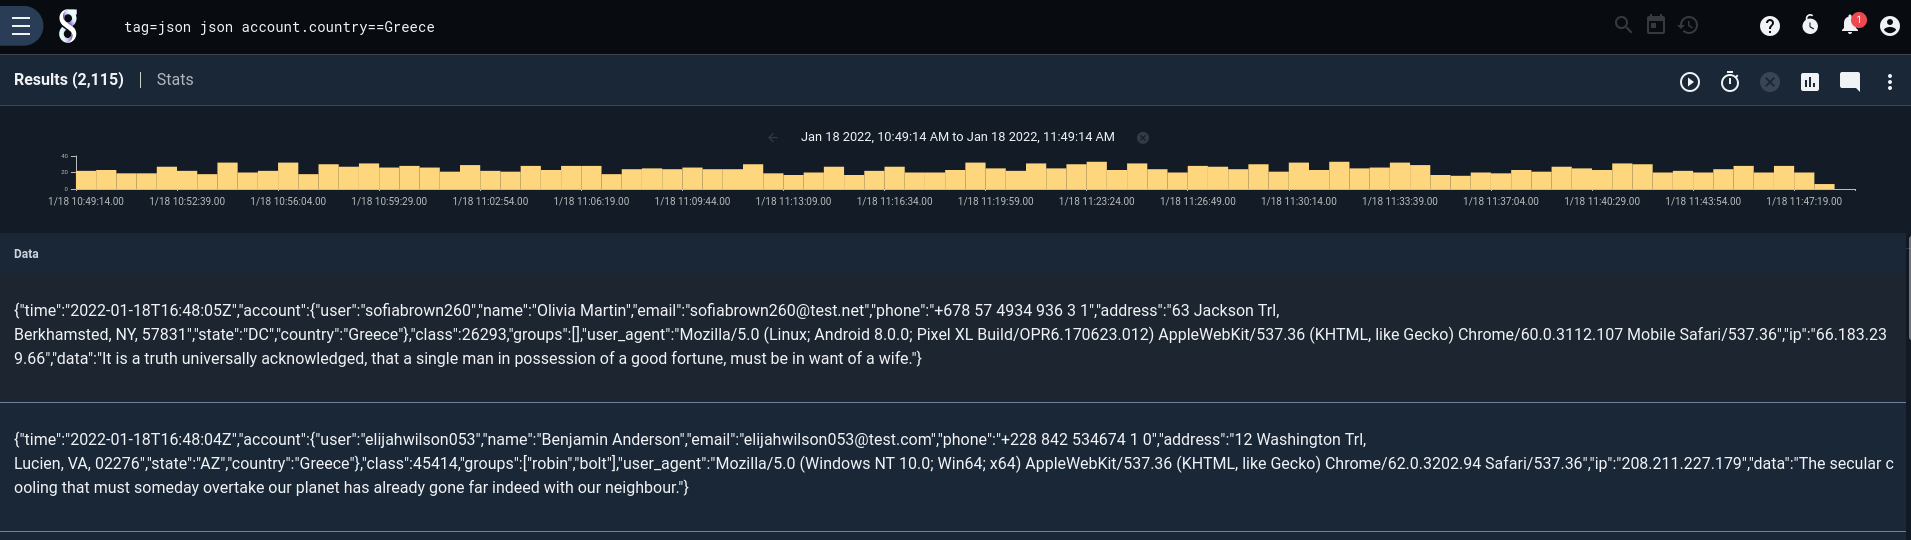
\includegraphics{images/greece-accel.png}
	\caption{Filtered Search Results}
	\label{fig:greece}
\end{figure}

Now click the stats tab on your results page to view the search stats, as shown in Figure \ref{fig:stats-accel}.
Pay special attention to the ``Entries processed'' value. That value
specifies how many entries actually entered the pipeline. Your dataset
contained 500k entries, but using the inline filtering and query
accelerators enabled you to only have to process a few thousand entries.
That's hundreds of thousands of entries that we didn't have to pull off
the disk or look at in any way.

\begin{figure}
	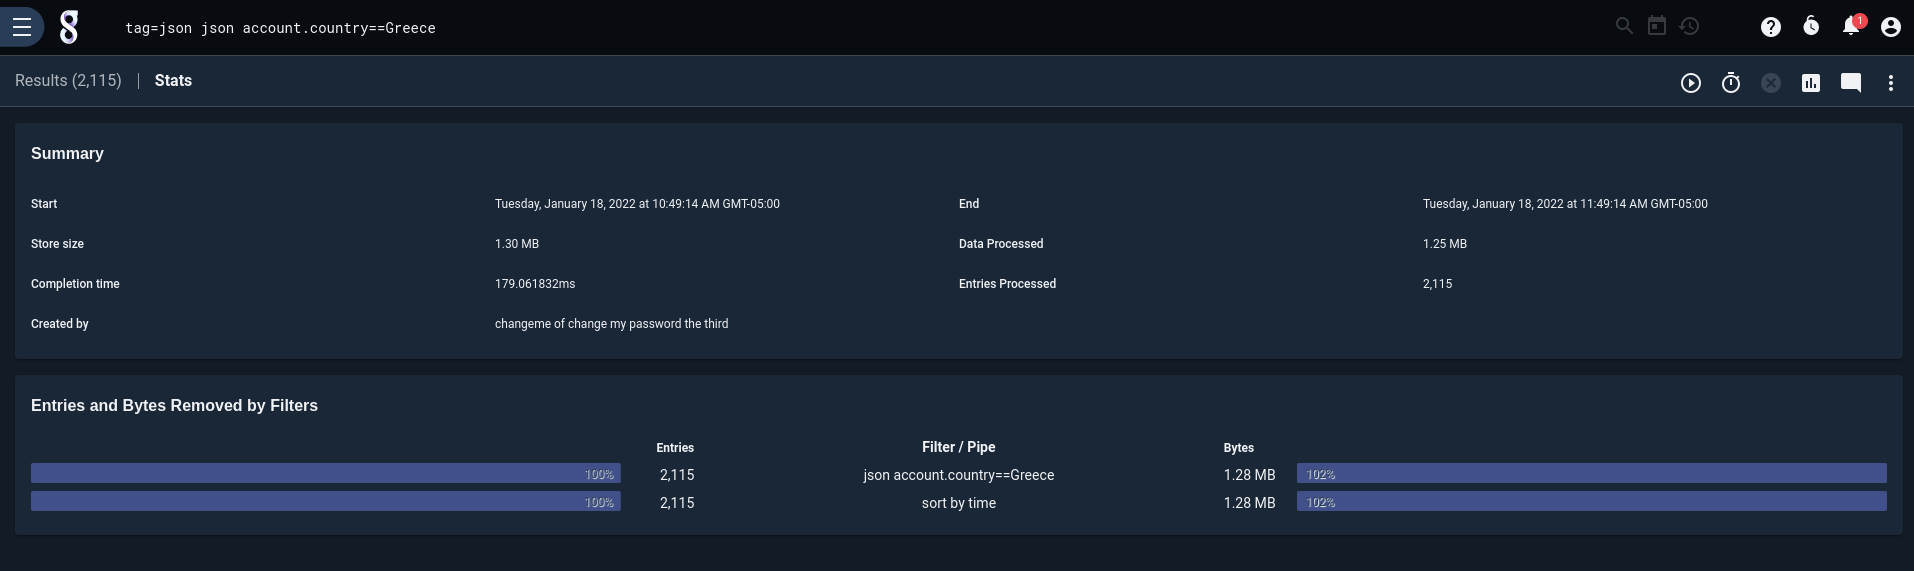
\includegraphics{images/stats-accel.png}
	\caption{Search Results Stats}
	\label{fig:stats-accel}
\end{figure}

\hypertarget{h.cpnsaxr7kale}{%
\subsubsection{\texorpdfstring{{}}{}}\label{h.cpnsaxr7kale}}

Next, we'll add two additional wells to the indexer.
The second well will enable query acceleration that is almost identical
to the well we have already configured, but instead of using the default
bloom engine, we are going to use the index engine. The third well will
not enable query acceleration at all.

Open your gravwell.conf file and add two additional wells with the
following parameters:

\begin{enumerate}
	\item Name: \code{json2}
	\begin{enumerate}
		\item Storage location \code{/opt/gravwell/storage/json2}
		\item Tag \code{json2} assigned
		\item \code{Accelerator-Name="json"}
		\item Extract the following fields: \code{class account.user account.email account.phone account.state account.country group ip}
		\item Set engine via \code{Accelerator-Engine-Override="index"} parameter
	\end{enumerate}
	\item Name: \code{json3}
	\begin{enumerate}
		\item Storage location \code{/opt/gravwell/storage/json3}
		\item Tag \code{json3} assigned
	\end{enumerate}
\end{enumerate}

Stop your gravwell container, copy the updated \code{gravwell.conf} file
into it, and then restart it:

\begin{Verbatim}[breaklines=true]
docker stop test
docker cp gravwell.conf test:/opt/gravwell/etc/gravwell.conf
docker start test
\end{Verbatim}

Re-ingest more JSON data using the tags ``json2'' and
``json3'':}

\begin{Verbatim}[breaklines=true]
docker run --net gravnet --rm -it gravwell:generators \
/jsonGenerator -clear-conns test -entry-count 500000 -tag-name json2
\end{Verbatim}

\begin{Verbatim}[breaklines=true]
docker run --net gravnet --rm -it gravwell:generators \
/jsonGenerator -clear-conns test -entry-count 500000 -tag-name json3
\end{Verbatim}

Go re-run the same query as before over a week, first using the tag
``json2'' then again using the tag ``json3'':

\begin{Verbatim}[breaklines=true]
tag=json2 json account.country==Greece
tag=json3 json account.country==Greece
\end{Verbatim}

You should get a few thousands results for each query,  but check the stats page and examine the
``Entries Processed'' results. For the tag \code{json3}, which used a well
that had no query acceleration, you should notice that the query had to
actually process 500k entries. That means the indexer had to get the
500k entries off the disk and put them in pipeline. The \code{json} module
was then responsible for performing all the filtering, meaning it had to
process every single entry. For the \code{json2} tag, you should notice
that the number of entries processed was the exact same as the number of
results. That is because the \code{index} engine doesn't have a high
statistical collision rate the way the \code{bloom} engine does. By reading
even fewer entries off the disk than with the bloom engine, this query is even faster.

\subsubsection{Lab Questions}

\begin{enumerate}
\item How much more storage did the bloom engine well consume than the raw well?
\item How much more storage did the index engine well consume than the bloom well?
\item What was the difference in ingest speed for each well?
\item How much faster was the index engine well than the bloom well?
\item And how much faster was the bloom well than the non-accelerated (raw) well?
\item If we re-run each query multiple times, how much faster was each?
	\begin{enumerate}
	\item Why?
	\item When would this NOT happen?
	\end{enumerate}
\end{enumerate}

To clean up after the experiment, simply run:

\begin{Verbatim}[breaklines=true]
docker kill $(docker ps -a -q)
\end{Verbatim}

\section{Indexer Optimization}
\index{Tuning!indexers}
Gravwell prides itself on not requiring specific machine specs and
being able to scale across a broad range of hardware capabilities.
While the software makes a best effort at scaling without human
intervention, there are several tuning parameters that can improve
storage and query efficiency on very large machines, and protect very
small machines from memory exhaustion. The tuning parameters are
focused on how the indexers organize discrete units of data and how
many of those units can be ``in flight'' at any given time. Varying
each parameter allows machines with lots of CPU cores and significant
memory to scale out and feed those cores as well as make more efficient
use of storage by effectively grouping data. Most default values are
geared towards a sane default that will operate well on a smaller
machine.

As data is ingested into a Gravwell indexer it is grouped in storage
units called blocks. The more efficiently that like data can be
colocated into blocks, the more efficient we can store and query data.
Gravwell indexers allow for fine tuning maximum block sizes and the
facilities used to generate those blocks.

\begin{figure}
	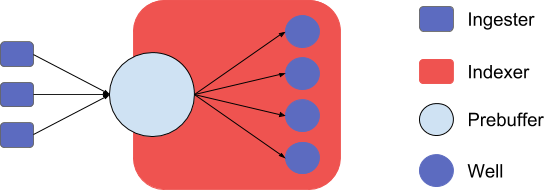
\includegraphics{images/prebuffer.png}
	\caption{Indexer Prebuffer}
	\label{fig:prebuffer}
\end{figure}

Each indexer employs a prebuffer (Figure \ref{fig:prebuffer}) used during ingest to hold a set of
incoming entries and organize them for better storage efficiency. The
prebuffer allows an indexer to tolerate ingesters that are sending
out-of-order data, or multiple ingesters with clock skews, while still
generating relatively efficient storage blocks. Large machines with
significant memory can allocate a larger prebuff to enable faster
ingest and better storage efficiency, while smaller machines with
limited memory can reduce the prebuffer so that more memory is available
for query.

Tuning block sizes is typically not required, but if you are operating
a very large cluster with very high data ingest rates, tuning the block
sizes can help query performance, compression efficiency, and ingest
throughput. By default indexers will store up to 4MB of data in a
single block. This means that if more than 4MB of data with the same
timestamp is ingested, it will be broken into multiple blocks. The
maximum block size is controlled using the \code{Max-Block-Size} parameter
in the global section of the \code{gravwell.conf} file. The size of a
block of can impact memory usage at query time, storage efficiency, and
compression efficiency. However, if you specify very large blocks and
large pipeline buffers, your indexer will consume significantly more
memory at query time and may not tolerate large numbers of concurrent
queries.

%%%%%%%%%%
% Commented this out because it's so esoteric.
% TODO: revisit, decide if we want it
%%%%%%%%%%
%\subsection{Hands-On Lab}
%
%For this hands on lab we are going to simulate a system with very high
%ingest rates and examine how various tuning parameters effect storage
%efficiency and ingest rates. We will create two wells which will
%receive roughly the same data. First we will ingest with a small
%prebuffer and small block sizes into one well, then we will reconfigure
%the prebuffer and block sizes to be much larger and ingest the same data
%again. We will examine how the storage sizes change and how query
%performance is affected. Due to the limited size of our test systems
%the results will not be terribly dramatic, but rest assured on very
%large clusters they can be.
%
%First let's change to our 4.5 directory and reset our environment:
%
%\begin{Verbatim}[breaklines=true]
%docker stop test
%docker rm test
%docker create --net gravnet --name test gravwell:base
%docker cp gravwell.conf test:/opt/gravwell/etc/gravwell.conf
%docker start test
%\end{Verbatim}
%
%Examine the \code{gravwell.conf} file. We have turned the block sizes and
%prebuffer sizes way down. Lets download a test data set and the single
%file ingester and push the data set into our test1 well using the
%\code{test1} tag.
%
%\begin{Verbatim}[breaklines=true]
%./bin/singleFile -i 4.5/data.gz -tag-name test1
%-clear-conns test
%\end{Verbatim}
%
%Make a note of the ingest rate and let's modify the gravwell.conf file
%to dramatically increase the prebuffer size, block size and block
%hints:
%
%\begin{Verbatim}[breaklines=true]
%Max-Block-Size=16
%Prebuff-Block-Hint=16
%Prebuff-Max-Size=64
%\end{Verbatim}
%
%Copy the gravwell.conf file back into your indexer, restart it, and
%ingest the same file again under the \code{test2} tag:
%
%\begin{Verbatim}[breaklines=true]
%docker cp gravwell.conf test:/opt/gravwell/etc/gravwell.conf
%docker restart test
%singleFile -i data.gz -tag-name test2 -clear-conns test
%\end{Verbatim}
%
%Compare the ingest rate using the new, larger pre-buffers with the
%original ingest rate, now examine the storage usage for each of the
%wells:
%
%\begin{Verbatim}[breaklines=true]
%docker exec -it test /bin/sh
%du -sh /opt/gravwell/storage/*
%exit
%\end{Verbatim}
%
%\subsubsection{Lab Questions}
%
%\begin{enumerate}
%\item Was there a difference in ingest performance?
%	\begin{enumerate}
%	\item Why?
%	\end{enumerate}
%\item Did the two wells consume different amounts of storage?
%	\begin{enumerate}
%	\item Why?
%	\end{enumerate}
%\item The indexes are different sizes (check the .accel directories), why?
%\end{enumerate}

\section{Docker Configuration}
\label{sec:docker-config}
\index{Docker}
Throughout the training so far we have made heavy use of Docker as a
simple container platform that makes it easy to configure and run
Gravwell. As you were working with Gravwell, there may have been a
nagging question about the gravwell.conf files we were using. There
were no secret tokens in any of them. The docs clearly state that you
MUST set the \code{Ingest-Secret} and \code{Control-Secret} parameters, but none of the
gravwell.conf files we have used so far have done so. Why? How have things
worked at all?

Docker is designed to rapidly deploy services with as little fanfare as
possible. Kubernetes and RedHat OpenShift build upon that concept and
take it to the extreme, making it possible to deploy extremely large
clusters of services with just a few commands. Configuring those
services with thousands of configuration files would be ridiculously
difficult, so the platforms provide a system called ``secrets'' which
allow you to inject environment variables and secure tokens into a
container at runtime. Those injected variables are how we have been
configuring the secrets: they were registered with the image and
injected every time you fired up a container. Check it by inspecting a
running gravwell:base container or image:

\code{docker inspect gravwell:base}

The pertinent section is \code{Config.Env}, which should contain the
following environment variables:

\begin{Verbatim}[breaklines=true]
GRAVWELL_INGEST_AUTH=IngestSecrets
GRAVWELL_INGEST_SECRET=IngestSecrets
GRAVWELL_CONTROL_AUTH=ControlSecrets
GRAVWELL_SEARCHAGENT_AUTH=SearchAgentSecrets
GRAVWELL_PIPE_TARGETS=/opt/gravwell/comms/pipe
\end{Verbatim}

Gravwell components will attempt to read configuration variables from
the \code{gravwell.conf} file, but if required variables are not present in
the config file it will look for them in the environment, and
optionally through Docker
secrets\footnote{https://docs.docker.com/engine/swarm/secrets/}. Gravwell
will only look at environment variables and/or secrets if the corresponding
gravwell.conf parameter is empty; the configuration file always
supersedes any environment or secret tokens. For more information see
our documentation section on Docker
configuration\footnote{https://docs.gravwell.io/\#!configuration/docker.md}

The environment variables associated with the image can be overridden
at runtime using the \code{-e} Docker flag. Remember that environment
variables are NOT a secure way to configure Gravwell, so if you are going
to use Docker, Kubernetes, or Openshift in production, use secrets
for the auth tokens.

\subsection{Hands-on Lab: Docker Configuration}

For this lab we are going to use Docker environment variables to stand
up a distributed 4-node Gravwell cluster in just a few commands without
fiddling with configuration files. We will inject all the needed
configuration parameters using Docker. If you are using a community
license you can complete the lab, but will only be able to configure a
single indexer.

Start by cleaning up your docker environment:

\begin{Verbatim}[breaklines=true]
docker stop test
docker rm test
\end{Verbatim}

Now look at \code{gravwell\_training/Indexers/Lab-Docker/config/gravwell.conf}
and note that we have removed the \code{Remote-Indexers}
configuration parameter so that we can inject a list of
indexers at runtime. First, fire up a container that is only running the
indexer, show the process list, and then clean up the container:

\begin{Verbatim}[breaklines=true]
docker create --net gravnet --name idx \
    -e DISABLE_WEBSERVER=TRUE -e DISABLE_SEARCHAGENT=TRUE \
    gravwell:base
docker cp gravwell.conf idx:/opt/gravwell/etc/
docker start idx
docker exec idx ps
docker stop idx
docker rm idx
\end{Verbatim}

You should see that only the \code{manager} and \code{gravwell\_indexer} processes are
running. The manager application is an open-source\footnote{https://github.com/gravwell/gravwell/tree/master/manager} Gravwell
process management application that somewhat takes on the role of
systemd. It respects some configuration via environment variables of its own.

\begin{Verbatim}[breaklines=true]
user@training:~$ docker exec -it idx ps
PID   USER     TIME  COMMAND
    1 root      0:00 /opt/gravwell/bin/manager
   11 root      0:00 /opt/gravwell/bin/gravwell_indexer -stderr indexer
   22 root      0:00 ps
user@training:~$
\end{Verbatim}

Now that we know how to start an indexer in a container without the
other services, let's fire up a few of them with a small loop. Make sure
you're in the \code{Indexers/Lab-Docker/config} directory, then run:

\begin{Verbatim}[breaklines=true]
for i in 1 2 3 4; do
    docker create --net gravnet --name idx$i \
    -e DISABLE_WEBSERVER=TRUE \
    -e DISABLE_SEARCHAGENT=TRUE \
    gravwell:base
docker cp gravwell.conf idx$i:/opt/gravwell/etc/
docker start idx$i
done
\end{Verbatim}

We should now have 4 indexers up and running, so let's start up the
webserver and configure it to connect to our indexers:

\begin{Verbatim}[breaklines=true]
docker create --net gravnet --name webserver \
    -e DISABLE_INDEXER=TRUE \
    -e GRAVWELL_REMOTE_INDEXERS=idx1,idx2,idx3,idx4 \
gravwell:base
docker cp gravwell.conf webserver:/opt/gravwell/etc/
docker start webserver
\end{Verbatim}

Get the webserver's IP address:

\begin{Verbatim}[breaklines=true]
docker inspect --format \
'{{.NetworkSettings.Networks.gravnet.IPAddress}}' webserver
\end{Verbatim}

Let's open up or Gravwell GUI and check out our indexer and hardware
tabs. You should see several indexers connected with a lot more
activity in the hardware monitoring page, as shown in Figures \ref{fig:idx-hardware} and \ref{fig:idx-wells}.

\begin{figure}
	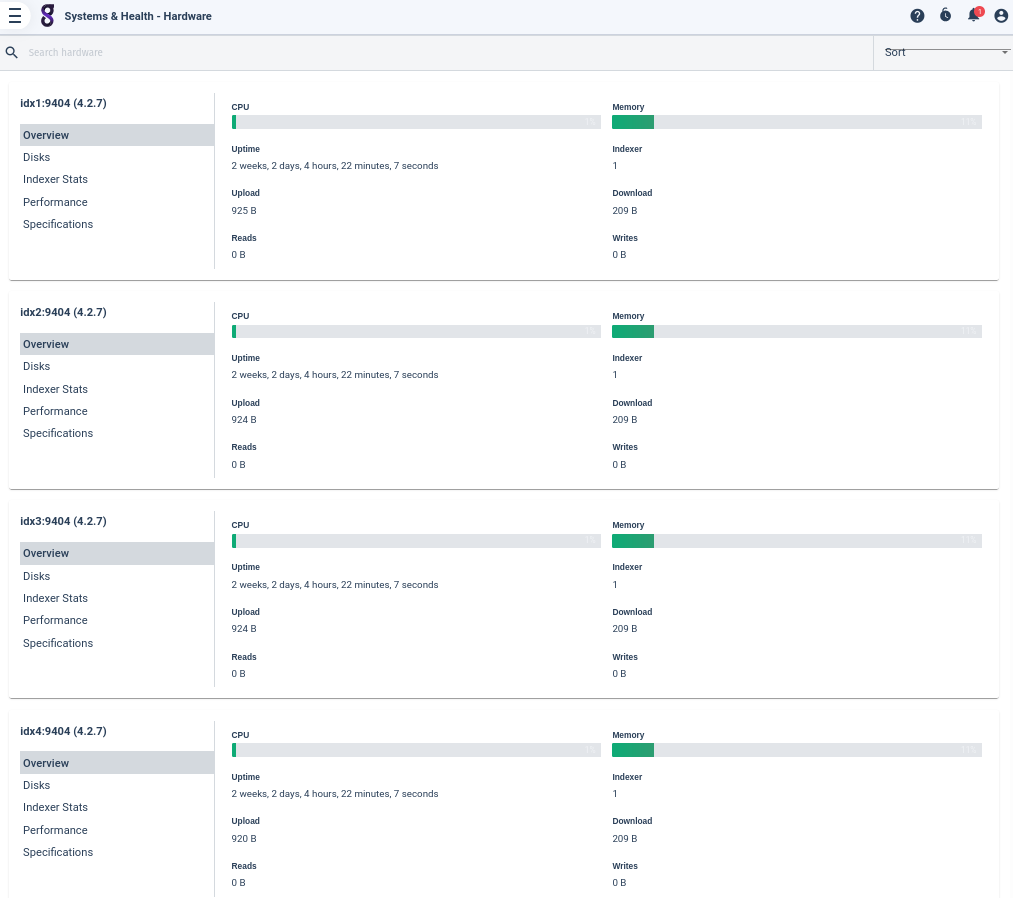
\includegraphics{images/hardware.png}
	\caption{Hardware Page with Four Indexers}
	\label{fig:idx-hardware}
\end{figure}

\begin{figure}
	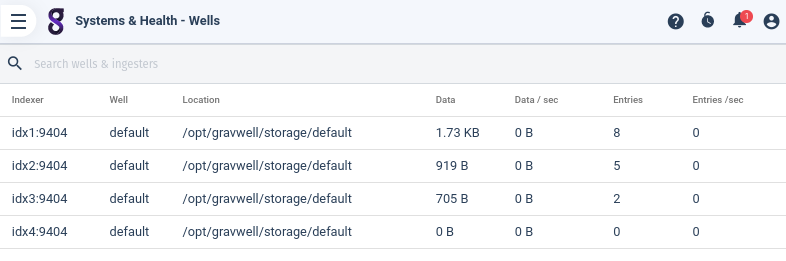
\includegraphics{images/docker-wells.png}
	\caption{Wells Page with Four Indexers}
	\label{fig:idx-wells}
\end{figure}

To clean up after the experiment, simply run:

\begin{Verbatim}[breaklines=true]
docker kill $(docker ps -a -q)
\end{Verbatim}
